% Options for packages loaded elsewhere
\PassOptionsToPackage{unicode}{hyperref}
\PassOptionsToPackage{hyphens}{url}
%
\documentclass[
]{article}
\usepackage{amsmath,amssymb}
\usepackage{setspace}
\usepackage{iftex}
\ifPDFTeX
  \usepackage[T1]{fontenc}
  \usepackage[utf8]{inputenc}
  \usepackage{textcomp} % provide euro and other symbols
\else % if luatex or xetex
  \usepackage{unicode-math} % this also loads fontspec
  \defaultfontfeatures{Scale=MatchLowercase}
  \defaultfontfeatures[\rmfamily]{Ligatures=TeX,Scale=1}
\fi
\usepackage{lmodern}
\ifPDFTeX\else
  % xetex/luatex font selection
\fi
% Use upquote if available, for straight quotes in verbatim environments
\IfFileExists{upquote.sty}{\usepackage{upquote}}{}
\IfFileExists{microtype.sty}{% use microtype if available
  \usepackage[]{microtype}
  \UseMicrotypeSet[protrusion]{basicmath} % disable protrusion for tt fonts
}{}
\makeatletter
\@ifundefined{KOMAClassName}{% if non-KOMA class
  \IfFileExists{parskip.sty}{%
    \usepackage{parskip}
  }{% else
    \setlength{\parindent}{0pt}
    \setlength{\parskip}{6pt plus 2pt minus 1pt}}
}{% if KOMA class
  \KOMAoptions{parskip=half}}
\makeatother
\usepackage{xcolor}
\usepackage[left=2cm,right=2cm,top=2cm,bottom=2cm]{geometry}
\usepackage{longtable,booktabs,array}
\usepackage{calc} % for calculating minipage widths
% Correct order of tables after \paragraph or \subparagraph
\usepackage{etoolbox}
\makeatletter
\patchcmd\longtable{\par}{\if@noskipsec\mbox{}\fi\par}{}{}
\makeatother
% Allow footnotes in longtable head/foot
\IfFileExists{footnotehyper.sty}{\usepackage{footnotehyper}}{\usepackage{footnote}}
\makesavenoteenv{longtable}
\usepackage{graphicx}
\makeatletter
\def\maxwidth{\ifdim\Gin@nat@width>\linewidth\linewidth\else\Gin@nat@width\fi}
\def\maxheight{\ifdim\Gin@nat@height>\textheight\textheight\else\Gin@nat@height\fi}
\makeatother
% Scale images if necessary, so that they will not overflow the page
% margins by default, and it is still possible to overwrite the defaults
% using explicit options in \includegraphics[width, height, ...]{}
\setkeys{Gin}{width=\maxwidth,height=\maxheight,keepaspectratio}
% Set default figure placement to htbp
\makeatletter
\def\fps@figure{htbp}
\makeatother
\setlength{\emergencystretch}{3em} % prevent overfull lines
\providecommand{\tightlist}{%
  \setlength{\itemsep}{0pt}\setlength{\parskip}{0pt}}
\setcounter{secnumdepth}{5}
\usepackage{lineno}
\linenumbers
\newcommand{\beginsupplement}{\setcounter{table}{0}  \renewcommand{\thetable}{S\arabic{table}} \setcounter{figure}{0} \renewcommand{\thefigure}{S\arabic{figure}}}
\usepackage{float}
\usepackage{booktabs}
\usepackage{caption}
\usepackage{longtable}
\usepackage{colortbl}
\usepackage{array}
\ifLuaTeX
  \usepackage{selnolig}  % disable illegal ligatures
\fi
\IfFileExists{bookmark.sty}{\usepackage{bookmark}}{\usepackage{hyperref}}
\IfFileExists{xurl.sty}{\usepackage{xurl}}{} % add URL line breaks if available
\urlstyle{same}
\hypersetup{
  pdftitle={IMF and Benchmark Forecasts},
  hidelinks,
  pdfcreator={LaTeX via pandoc}}

\title{IMF and Benchmark Forecasts}
\author{}
\date{\vspace{-2.5em}}

\begin{document}
\maketitle

\setstretch{2}
\hypertarget{extracting-error-quantiles}{%
\section{Extracting error quantiles}\label{extracting-error-quantiles}}

Consider a forecast that stems from a source \(s\) for a specific target \(k\) in a country \(j\), for target year \(t\) and with forecast horizon \(h\):
\[
\hat{y}_{s,k,j,t,h}
\]
For example, this could be a forecast stemming from the International Monetary Fund World Economic Outlook (\(s = IMF\)) for real GDP growth (\(k = gdpg\)) in Canada (\(j = Canada\)) for the year \(2022\) (\(t=2022\)). \(h\) then indexes the forecast horizon, where we code:
\[
h = \left\{
\begin{array}{ll} 
      0, & \textrm{for forecasts made in October of the same year} \\
      0.5, & \textrm{for forecasts made in April of the same year} \\
      1, & \textrm{for forecasts made in October of the previous year} \\
      1.5, & \textrm{for forecasts made in April of the previous year} \\
\end{array}\right. 
\]
After the target year has completed, we obtain the realized value for the quantity of interest. For these, the WEO updates publishes biannual updates for two years, yielding \(4\) versions of the realized value. In accordance with previous literature (\textit{cite Timmermann 2008}), we use the version that is published in October of the following year and thereby don't index the true value by its publishing date (\textit{rephrase}). We thus write the true value as
\[
\hat{y}_{k,j,t}
\]
Given the forecast and the realized value for the quantity of interest, we can calculate the respective forecast error as
\[
e^{d}_{s,k,j,t,h} = y_{k,j,t} - \hat{y}_{s,k,j,t,h}
\]

for the ``directional'' error method and as
\[
e^{a}_{s,k,j,t,h} = \left|y_{k,j,t} - \hat{y}_{s,k,j,t,h}\right|
\]
for the ``absolute'' error method.

The objective is to extract quantiles from sets of errors \(\mathcal{E}_{s,k,j,t,h}\) constructed of certain years, depending on the estimation method \(m\), to be able to quantify the uncertainty inherent in the forecasts via central prediction intervals of level \(\alpha = \{0.5, 0.8\}\). For the estimation method, we consider a ``rolling window'' method, an ``expanding window'' method, and a ``leave-one-out'' method. For the rolling window method (\(m = rw\)), the errors of the last nine years enter into the estimation. For the expanding window method (\(m = ew\)), all previous years are considered, leaving a nine year window up front for the first estimation. For the leave-one-out method, all years except the current target year enter the estimation set. The latter is of course equivalent to the expanding window method in a real time setting and is considered in the scope of this analysis as a mere check \textit{rephrase}.
As an example, the error set for the ``directional'' error method and the rolling window approach is
\[
\mathcal{E}^{d,rw}_{s,k,j,t,h} =  \left\{  e^{d}_{s,k,j,t^*,h} | t-9\leq t^* < t \right\}
\]
Insert reasoning to use the past \(9\) errors.

To now obtain the lower \(l\) and upper \(u\) values for a central prediction interval of level \(\alpha\), we take quantiles of these sets and add them to the current prediction:

For the directional method:
\[
l^{\alpha, d}_{t,h,v,l,j} = \hat{y}_{t, h, l, j} + q^{0.5 - \alpha/2 } \left(\mathcal{E}^{d, m}_{t,h,v,l,j}  \right)
\]
\[
u^{\alpha, d}_{t,h,v,l,j} = \hat{y}_{t, h, l, j} + q^{0.5 + \alpha/2 } \left(\mathcal{E}^{d, m}_{t,h,v,l,j}  \right)
\]

And for the absolute method:

\[
 l^{\alpha, a}_{t,h,v,l,j} = \hat{y}_{t, h, l, j} -  q^{\alpha} \left(\mathcal{E}^{m, a}_{t,h,v,l,j}  \right)
\]
\[
u^{\alpha, a}_{t,h,v,l,j} = \hat{y}_{t, h, l, j} +  q^{\alpha} \left(\mathcal{E}^{m, a}_{t,h,v,l,j}  \right)
\]

Two different philosophies.

The absolute method will always yield symmetric central prediction intervals around the forecast value, while the directional method will in general yield asymmetric intervals. They thus result in different central intervals, unless the errors in \(\mathcal{E}\) are perfectly symmetric around zero\footnote{Not totally correct, actually. For this to hold exactly, the error set would need to be augmented with one zero value.}. In fact, the directional method can yield central prediction intervals that do not even contain the forecast value, in cases where the \((0.5 - \alpha/2)\)-quantile is positive or the \((0.5 + \alpha/2)\)-quantile is negative.

\hypertarget{scores-by-error-method-horizon-and-forecast-source}{%
\section{Scores, by error method, Horizon and forecast source}\label{scores-by-error-method-horizon-and-forecast-source}}

\hypertarget{inflation}{%
\subsection{Inflation}\label{inflation}}

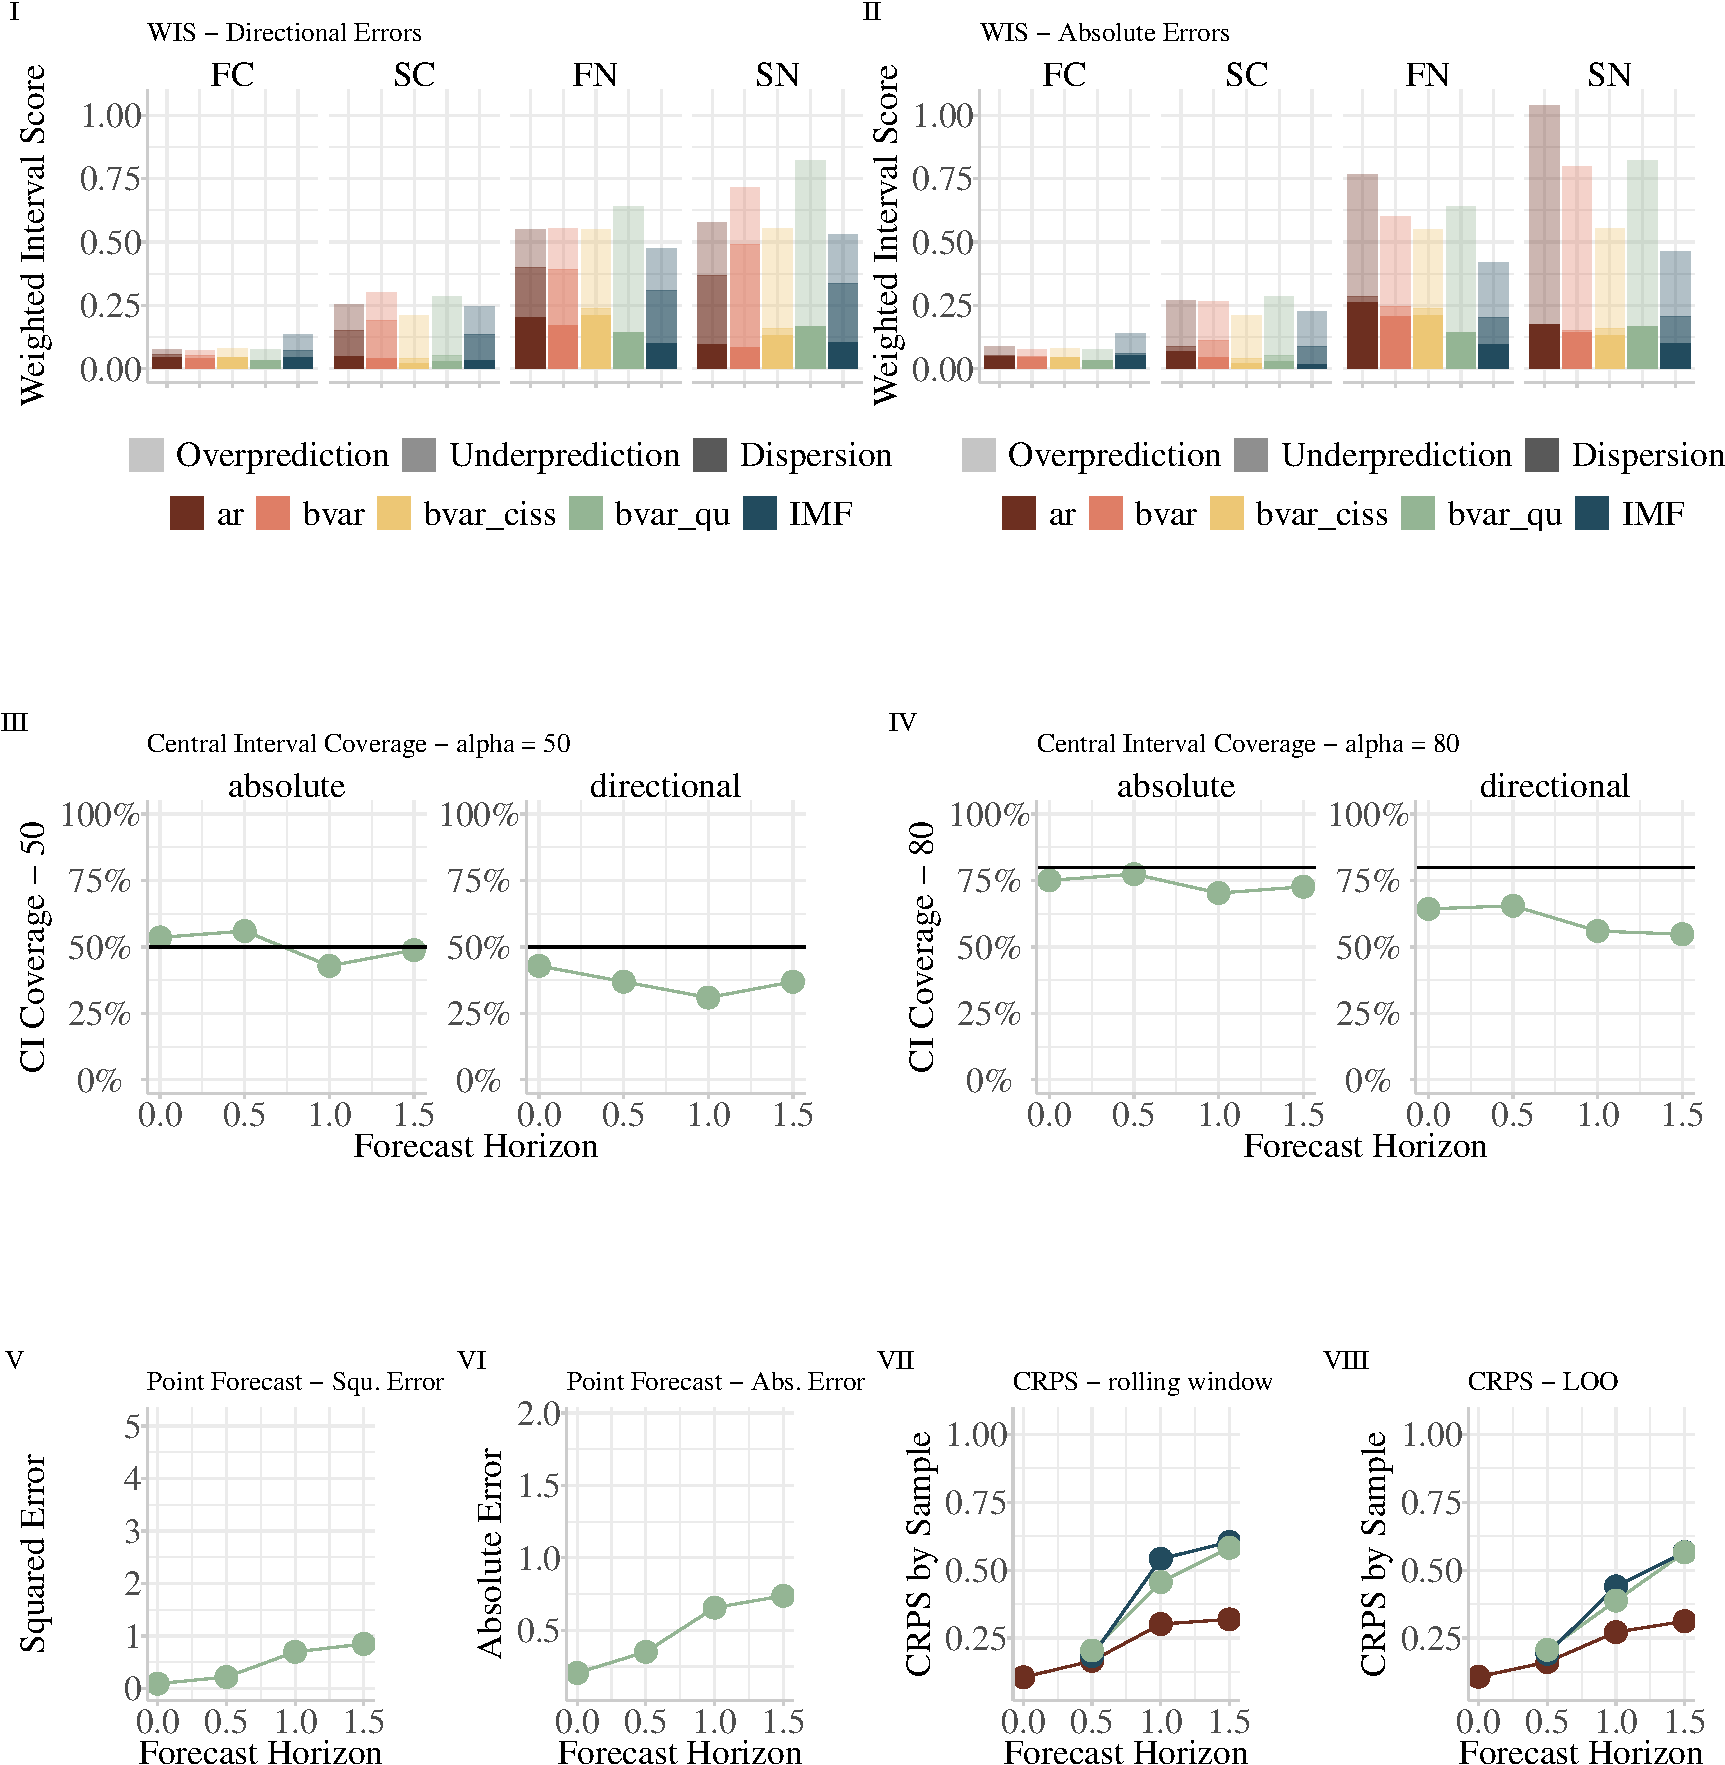
\includegraphics{manuscript_files/figure-latex/overall_assessment_ew-1.pdf}
\newpage
Some notes:

\begin{itemize}
\item Inflation: directional vs. absolute errors:
\begin{itemize}
\item difference small for IMF method, absolute slightly better, likely due to longer central intervals
\item AR and BVAR profit more from directional correction (upward bias)
\item for expanding window method, difference in coverage is smaller (-> structural breaks)

\end{itemize}
\item Inflation overall scores: IMF forecasts outperform others
\begin{itemize}
\item lower scores for point forecasts
\item lower WIS 
\item lower bias (compute directly?)
\end{itemize}


\item GDP Growth: more similar results for different sources
\begin{itemize}
\item lower scores at shorter horizons, more similar at larger horizons
\item IMF forecasts better only for absolute error method
\end{itemize}
\end{itemize}

\newpage

\hypertarget{gdp}{%
\subsection{GDP}\label{gdp}}

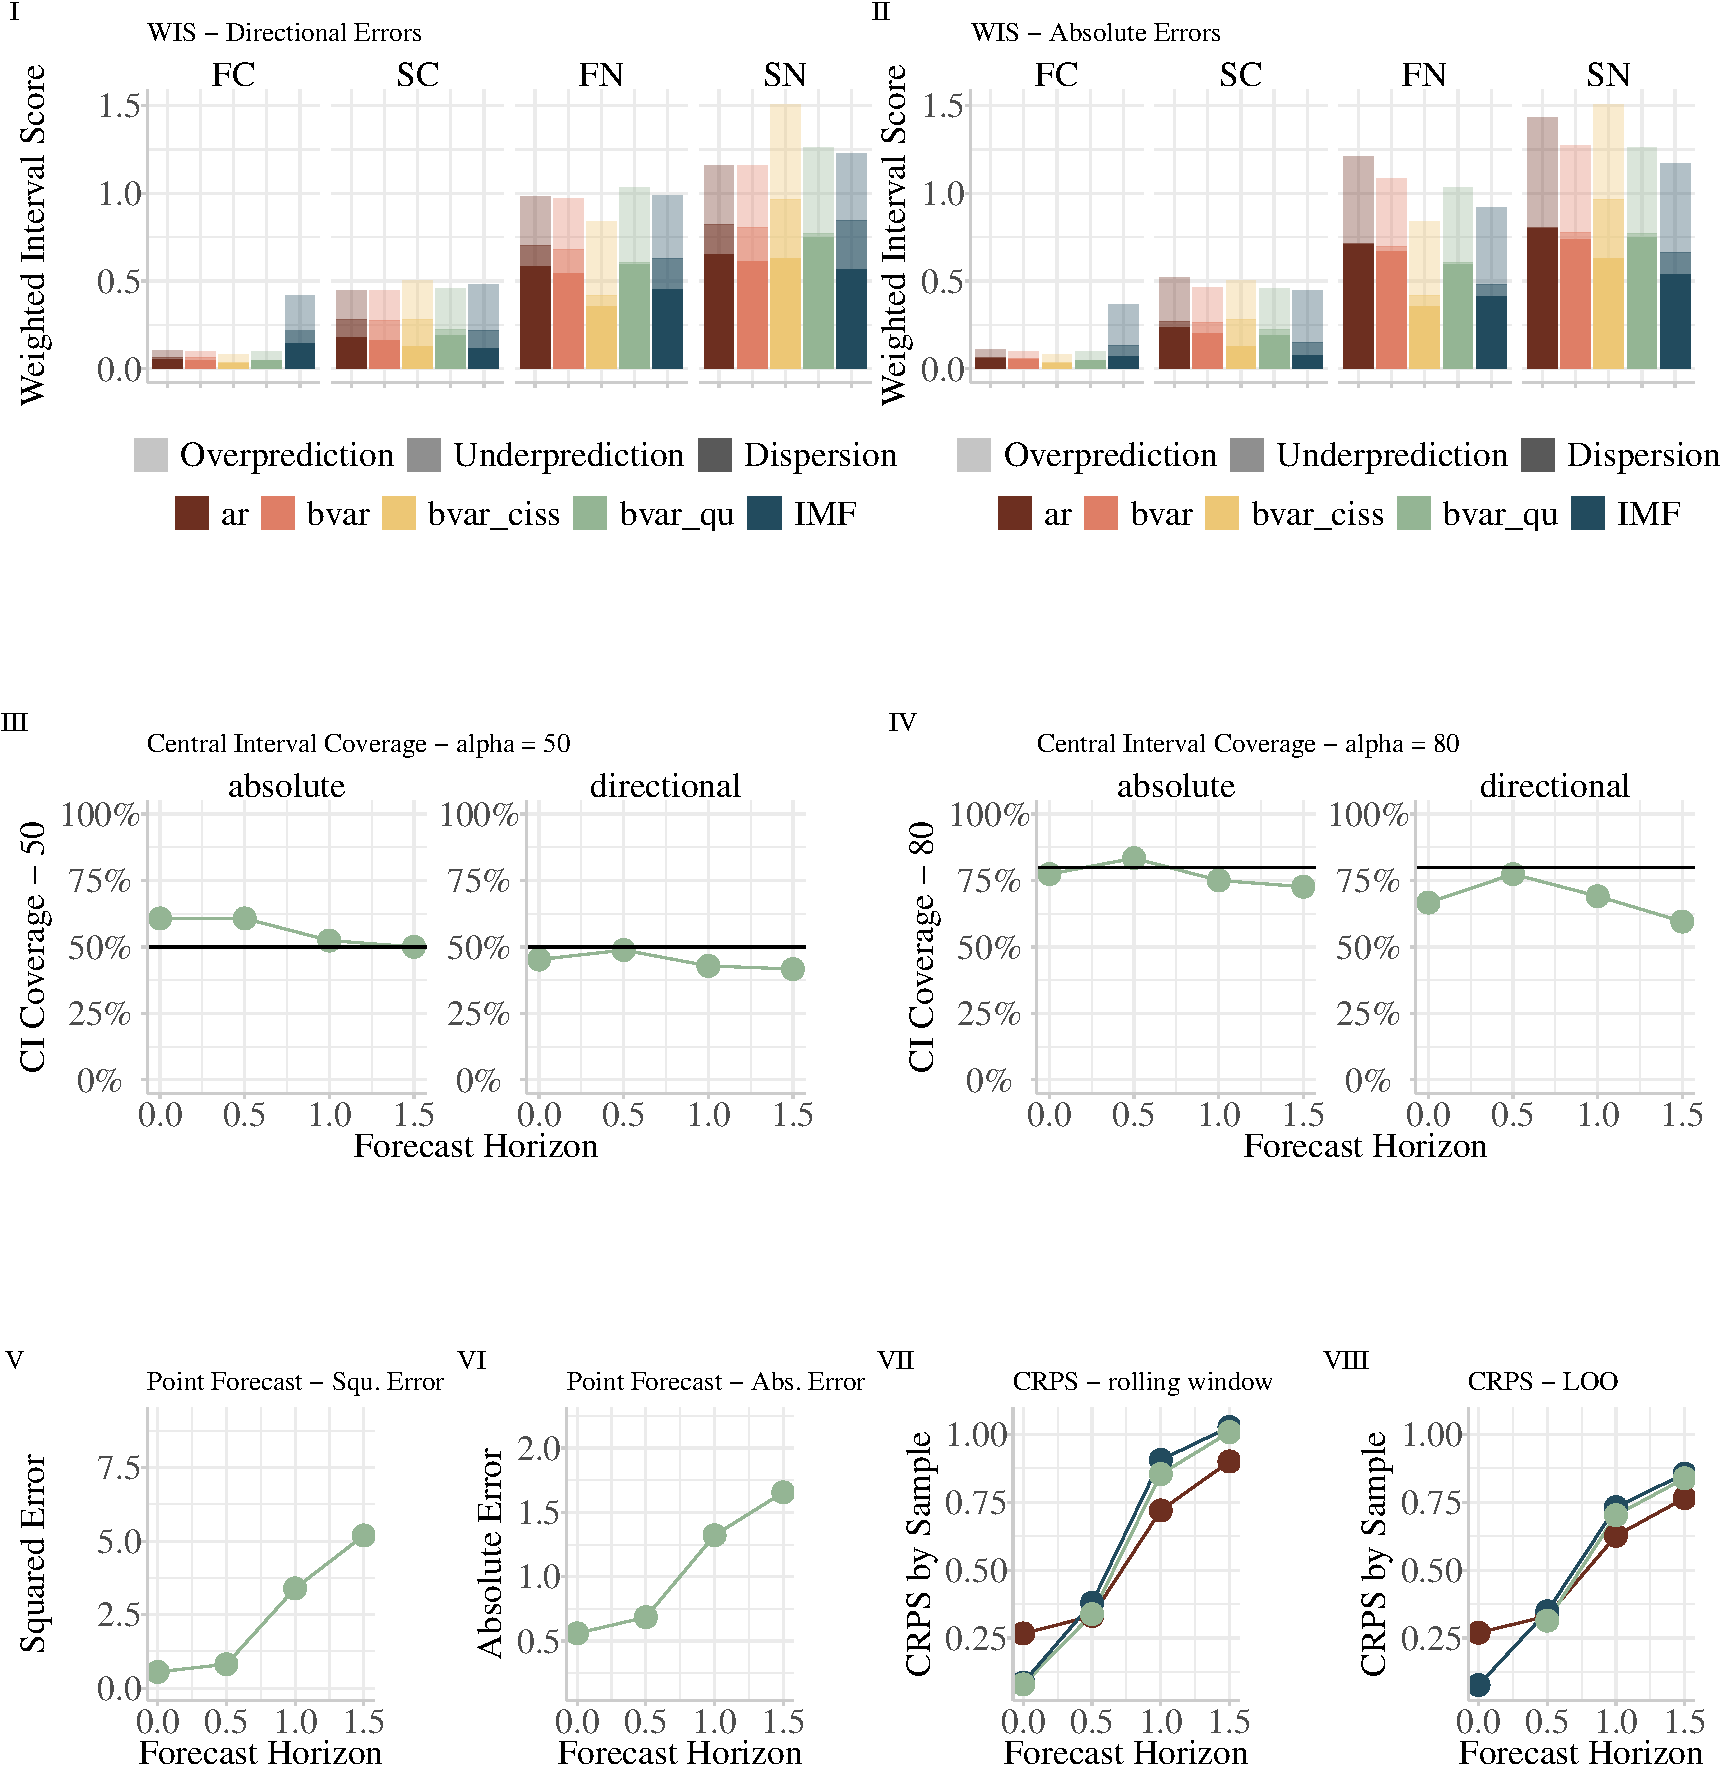
\includegraphics{manuscript_files/figure-latex/gdpovr_rw-1.pdf}

\hypertarget{expanding-window---scores-by-error-method-horizon-and-forecast-source}{%
\section{Expanding Window - Scores, by error method, Horizon and forecast source}\label{expanding-window---scores-by-error-method-horizon-and-forecast-source}}

\hypertarget{inflation-1}{%
\subsection{Inflation}\label{inflation-1}}

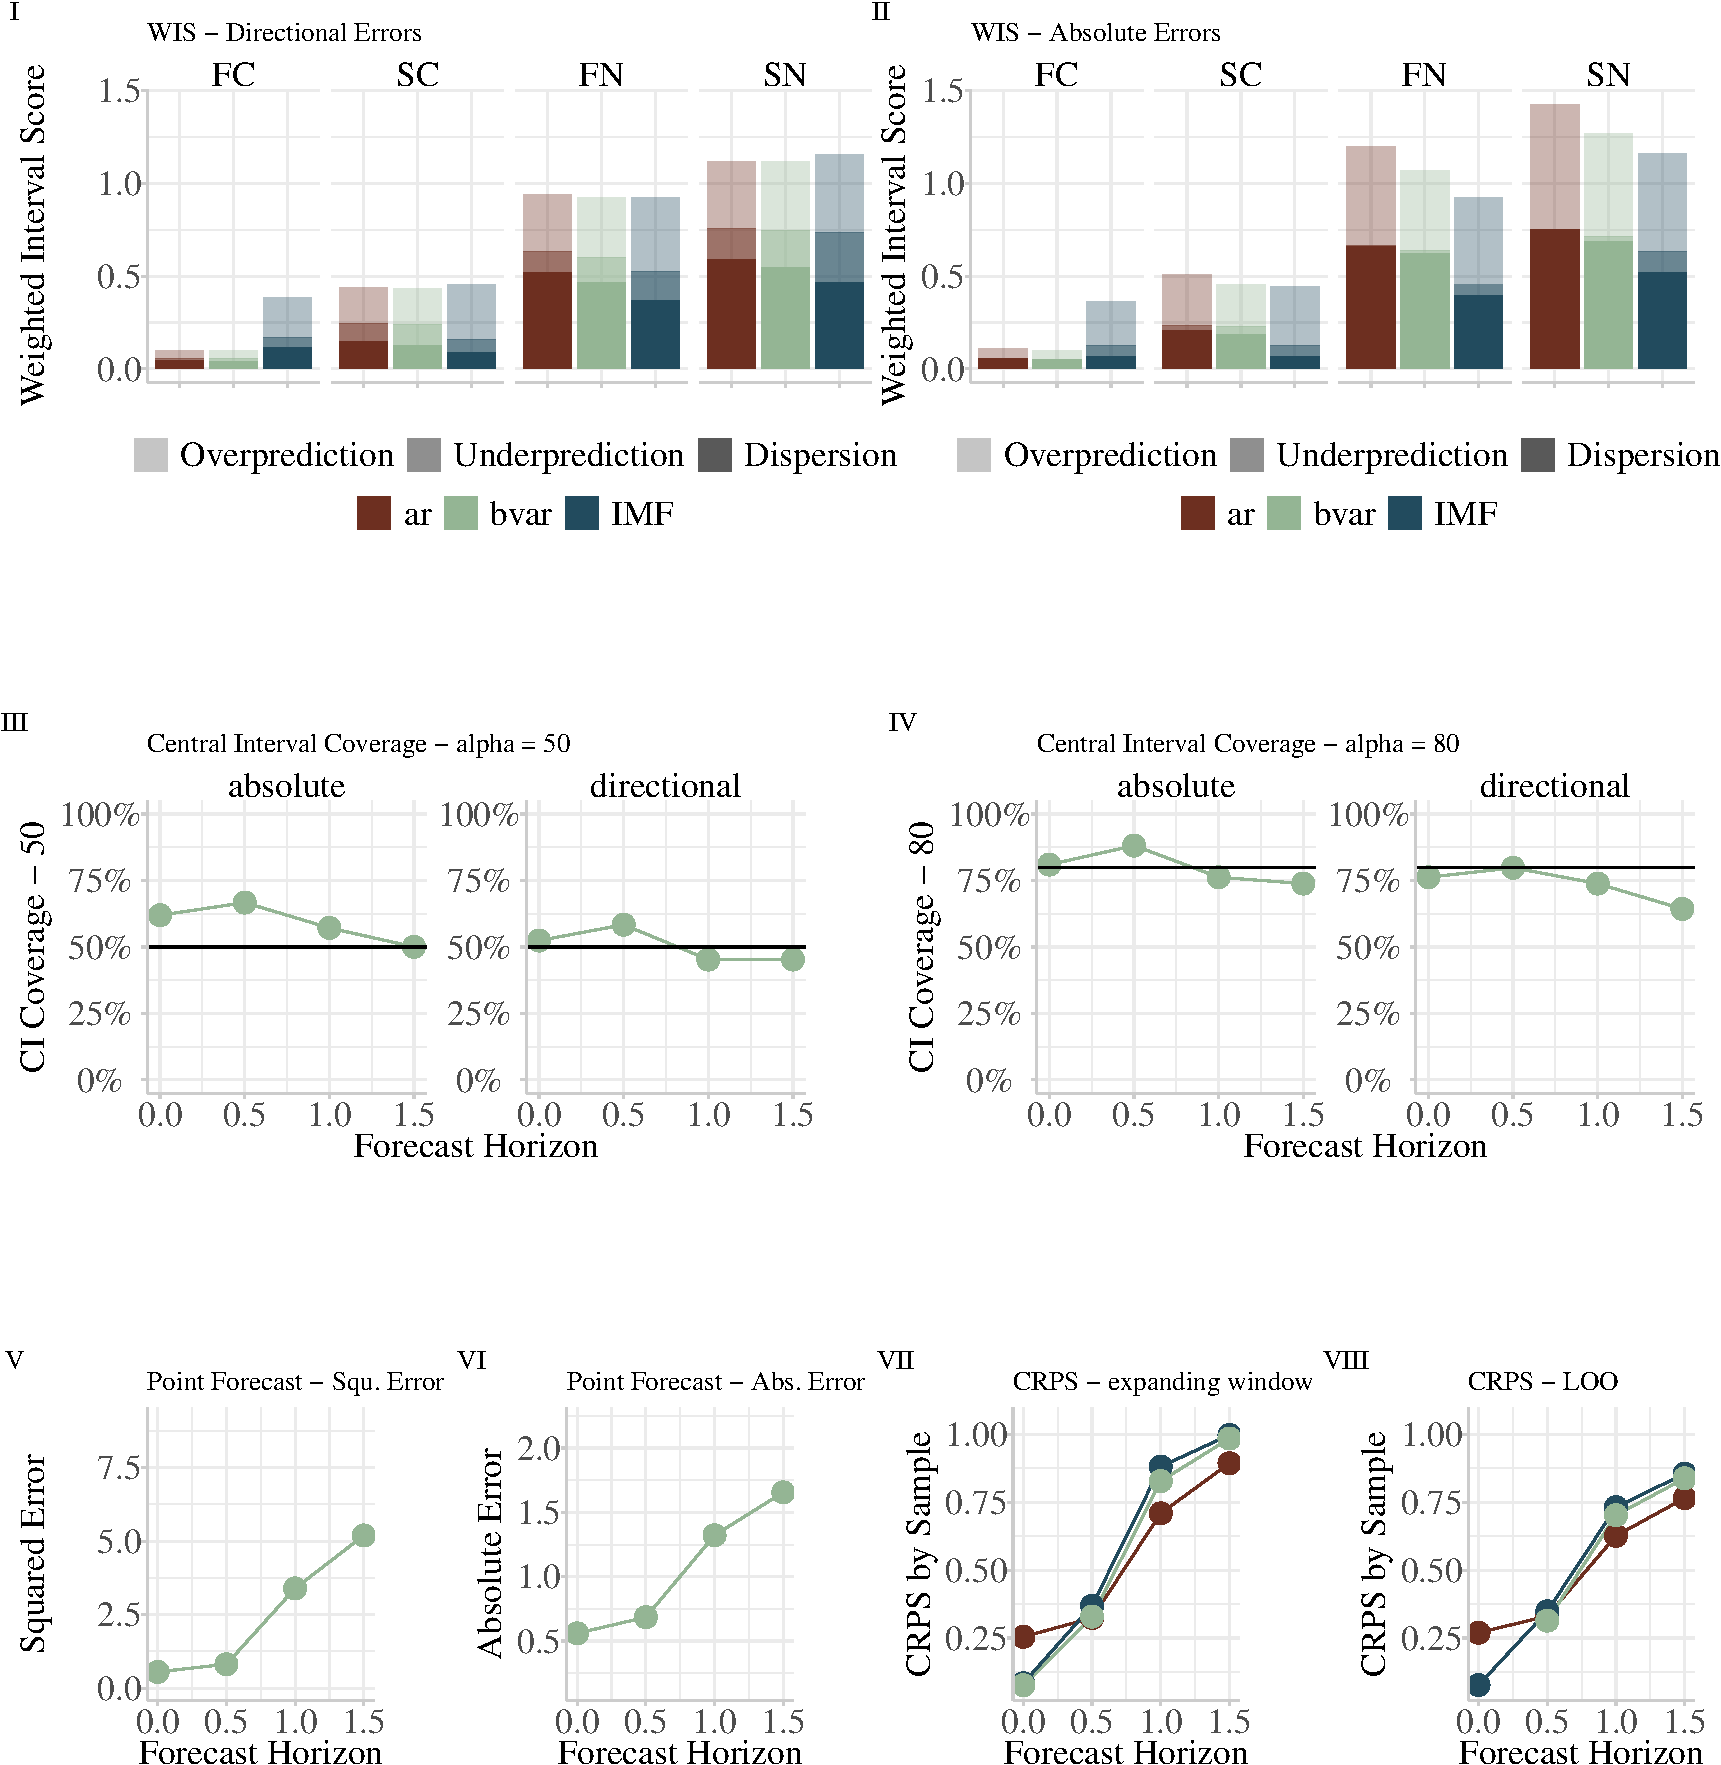
\includegraphics{manuscript_files/figure-latex/infklovr_ew-1.pdf}

\newpage

\hypertarget{gdp-1}{%
\subsection{GDP}\label{gdp-1}}

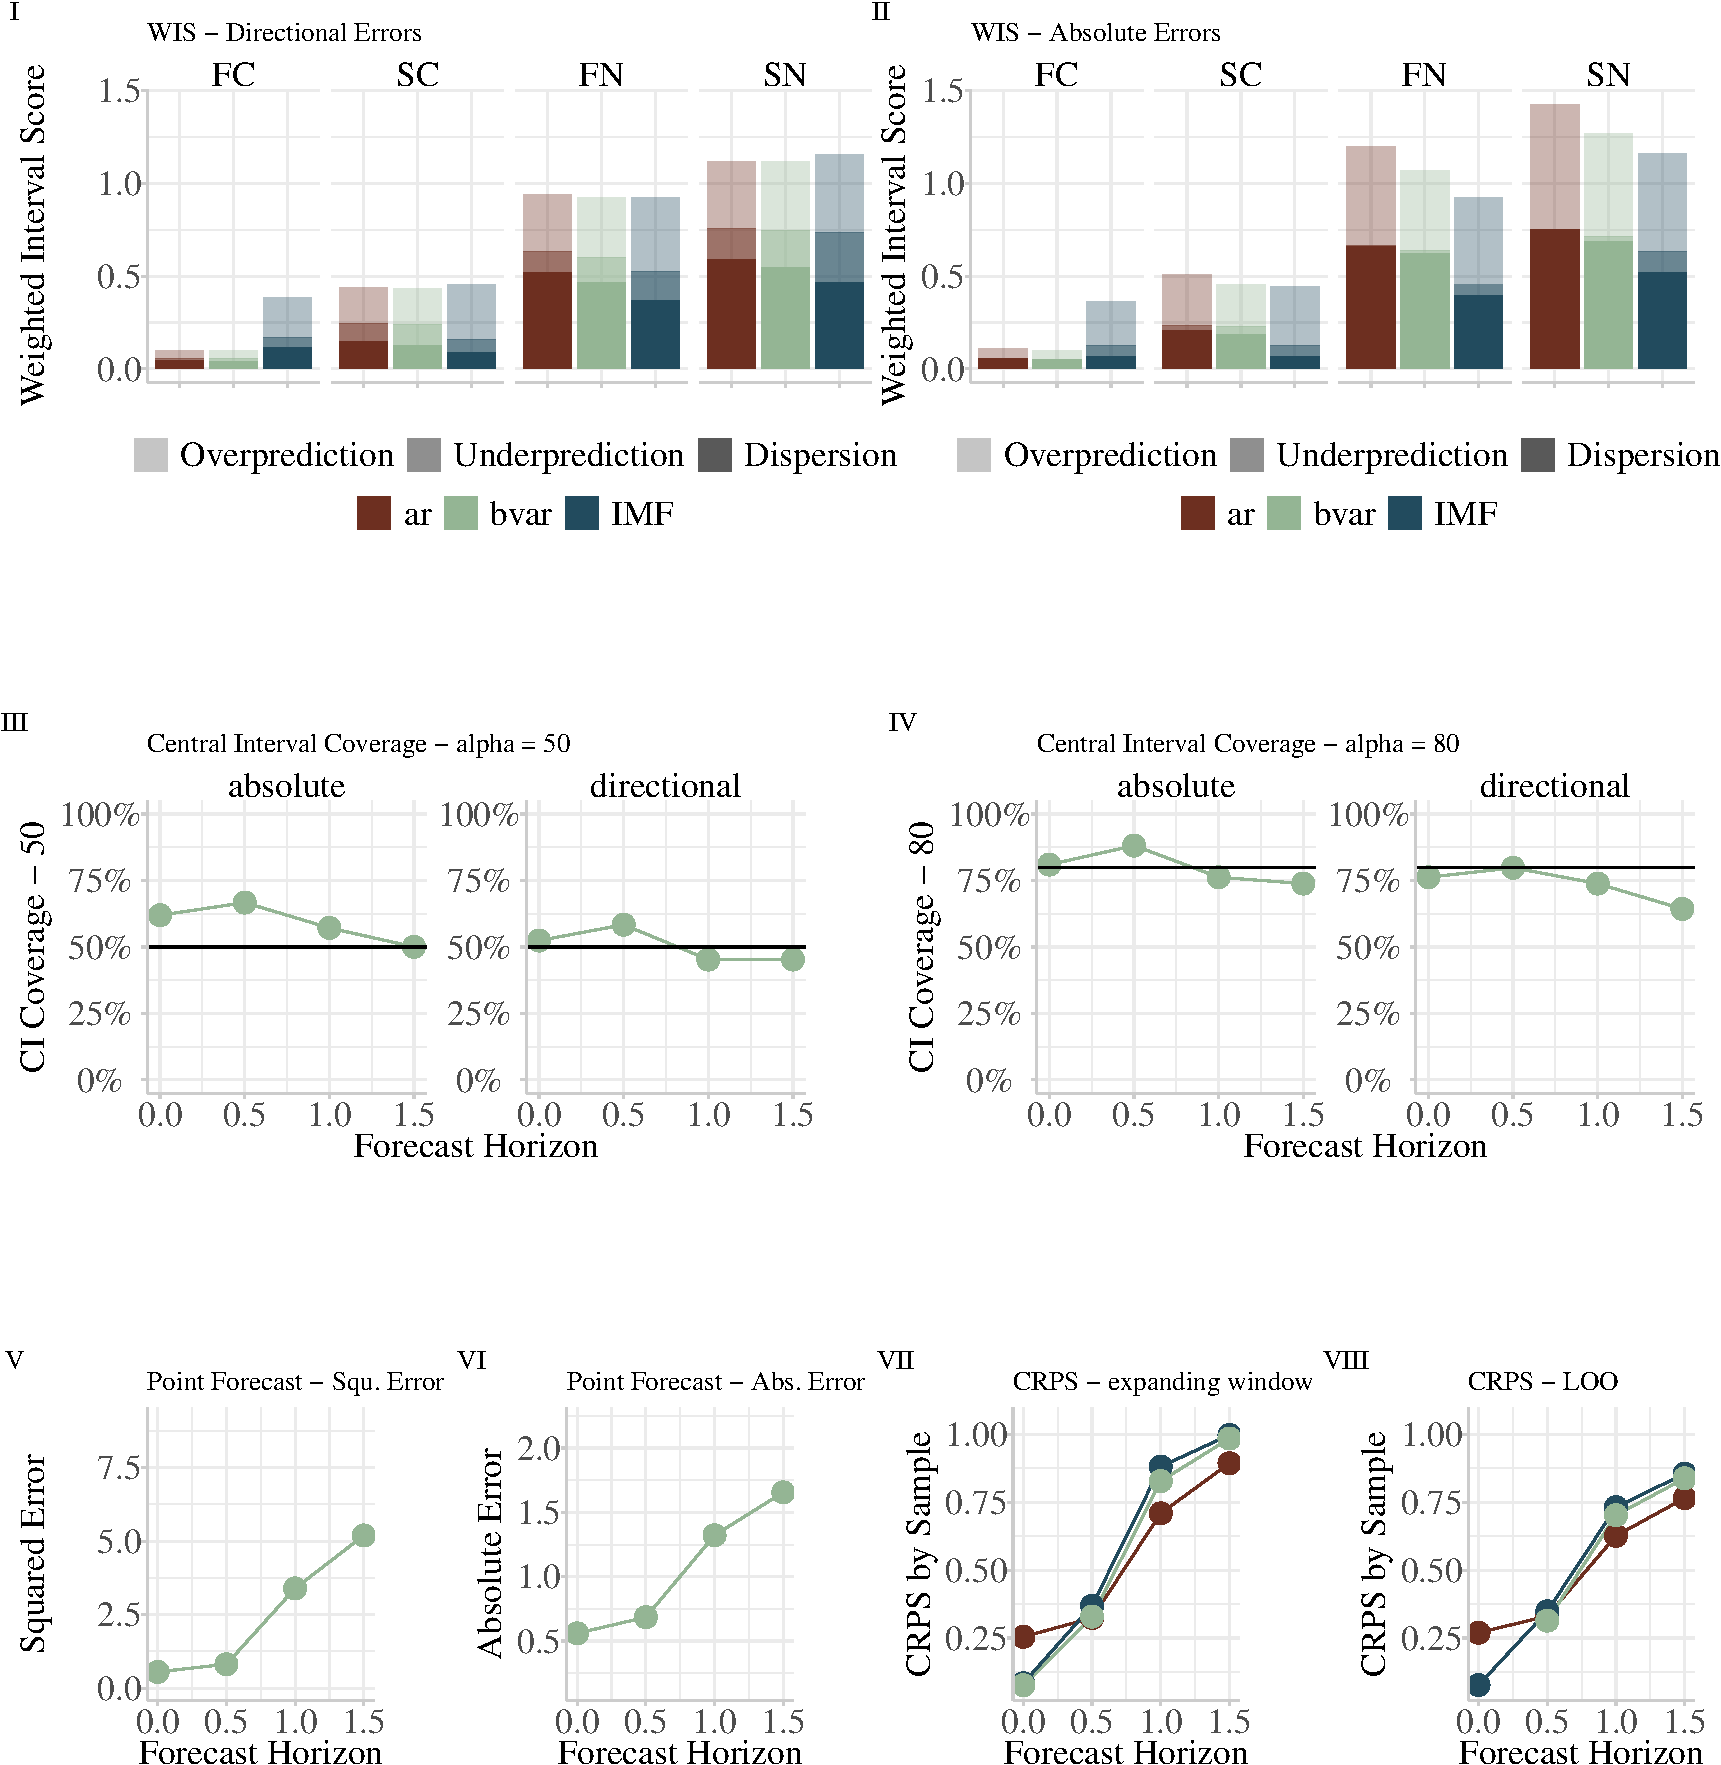
\includegraphics{manuscript_files/figure-latex/gdpovr-1.pdf}

\hypertarget{coverage-by-target-methods-and-source}{%
\section{Coverage, by target, methods and source}\label{coverage-by-target-methods-and-source}}

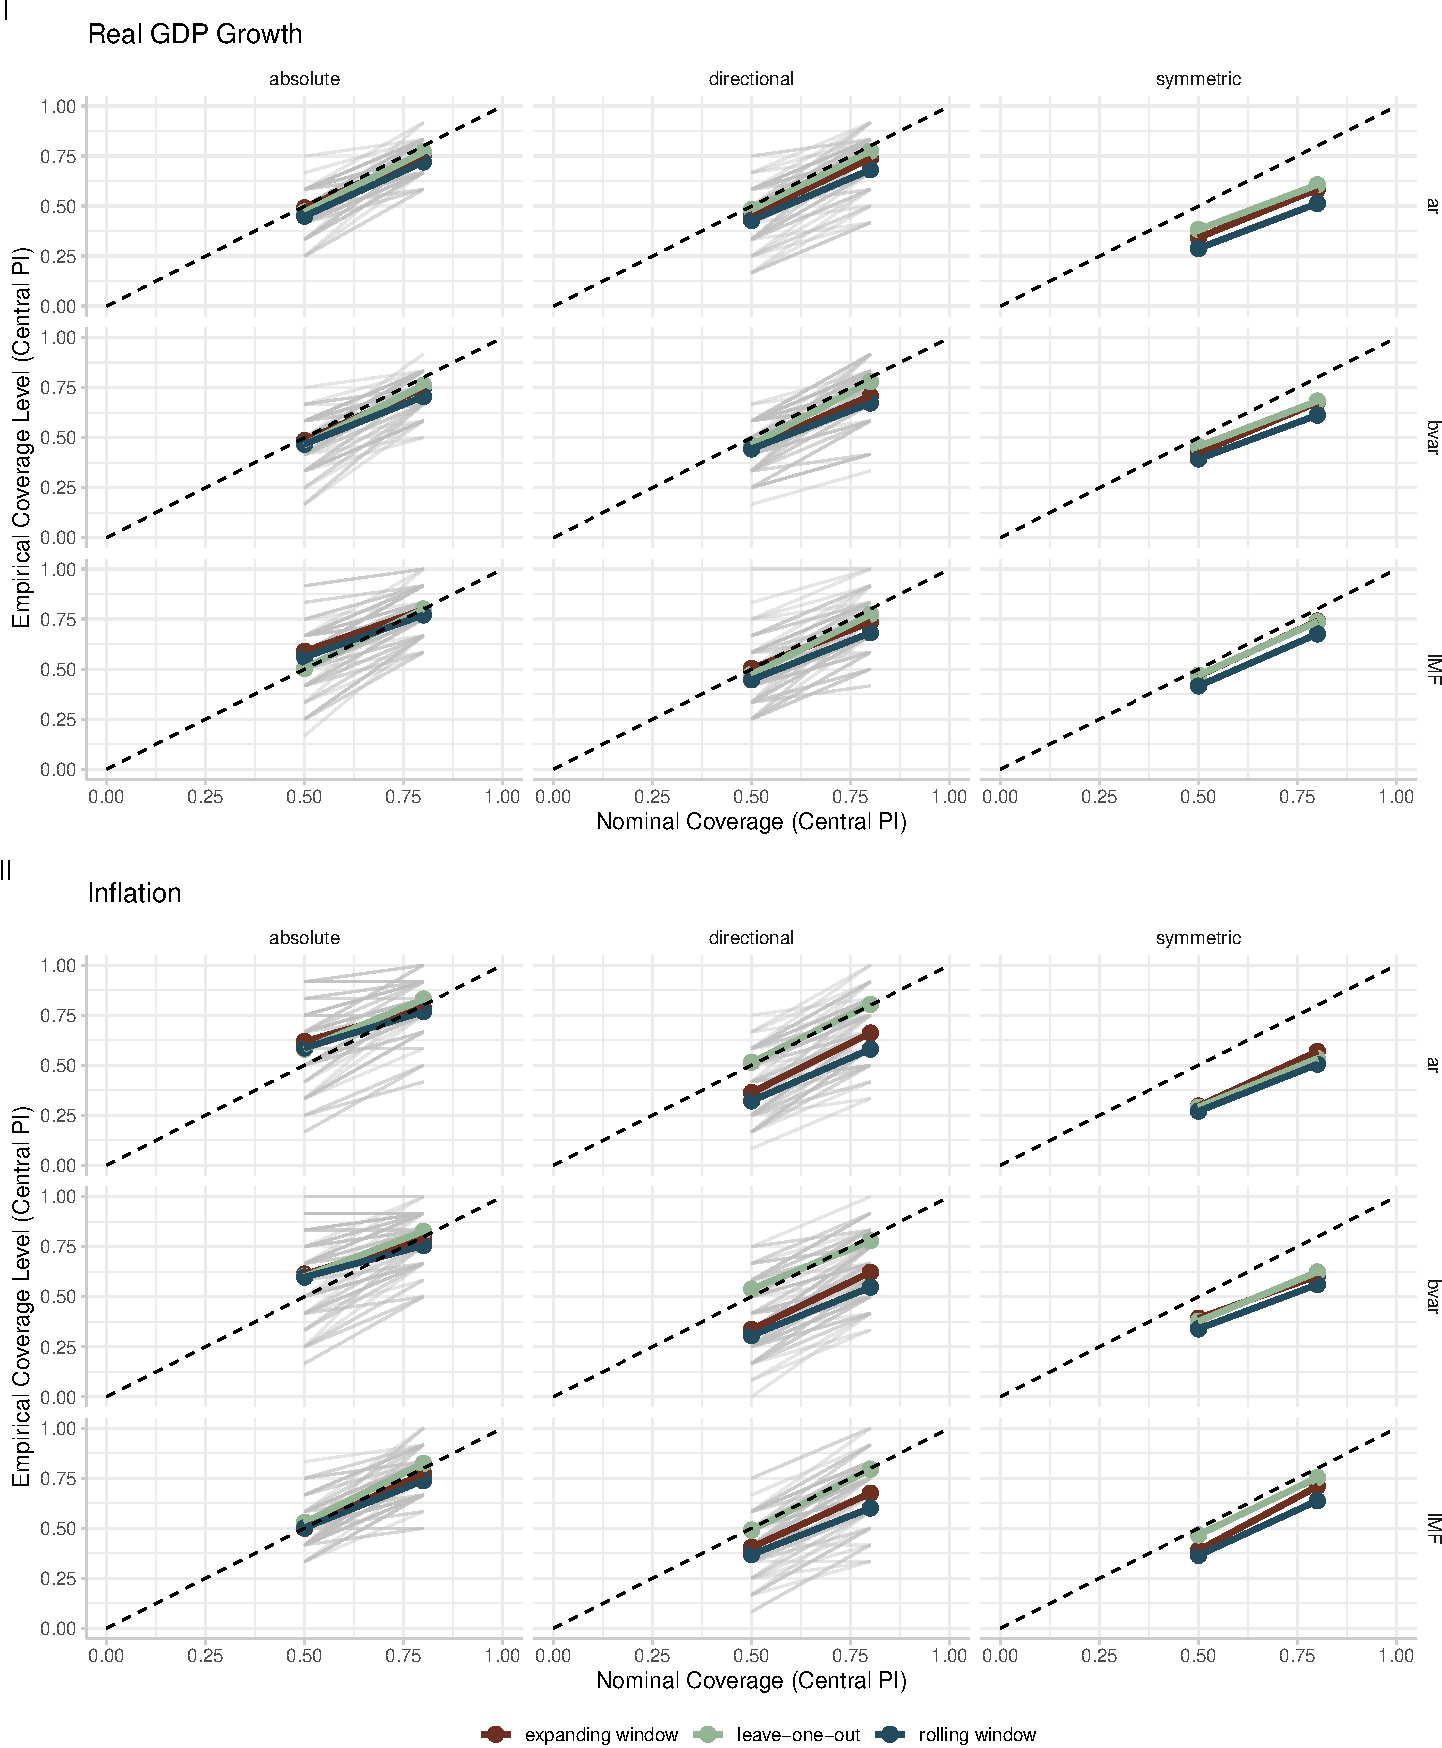
\includegraphics{manuscript_files/figure-latex/cvgplot-1.pdf}

\newpage
\begin{longtable}{l|rrr}
\toprule
\multicolumn{1}{l}{} & IMF & ar & bvar \\ 
\midrule\addlinespace[2.5pt]
\multicolumn{4}{l}{horizon = 0} \\ 
\midrule\addlinespace[2.5pt]
expanding window\_interval\_score & 0.115 & 0.123 & 0.122 \\ 
expanding window\_sample\_crps & 0.087 & 0.092 & 0.091 \\ 
leave-one-out\_interval\_score & 0.112 & 0.123 & 0.123 \\ 
leave-one-out\_sample\_crps & 0.088 & 0.099 & 0.100 \\ 
rolling window\_interval\_score & 0.119 & 0.128 & 0.126 \\ 
rolling window\_sample\_crps & 0.094 & 0.097 & 0.098 \\ 
\midrule\addlinespace[2.5pt]
\multicolumn{4}{l}{horizon = 0.5} \\ 
\midrule\addlinespace[2.5pt]
expanding window\_interval\_score & 0.258 & 0.272 & 0.296 \\ 
expanding window\_sample\_crps & 0.182 & 0.208 & 0.241 \\ 
leave-one-out\_interval\_score & 0.257 & 0.257 & 0.276 \\ 
leave-one-out\_sample\_crps & 0.180 & 0.217 & 0.230 \\ 
rolling window\_interval\_score & 0.261 & 0.266 & 0.288 \\ 
rolling window\_sample\_crps & 0.191 & 0.201 & 0.235 \\ 
\midrule\addlinespace[2.5pt]
\multicolumn{4}{l}{horizon = 1} \\ 
\midrule\addlinespace[2.5pt]
expanding window\_interval\_score & 0.447 & 0.740 & 0.595 \\ 
expanding window\_sample\_crps & 0.327 & 0.504 & 0.426 \\ 
leave-one-out\_interval\_score & 0.443 & 0.746 & 0.587 \\ 
leave-one-out\_sample\_crps & 0.302 & 0.448 & 0.400 \\ 
rolling window\_interval\_score & 0.458 & 0.744 & 0.601 \\ 
rolling window\_sample\_crps & 0.333 & 0.514 & 0.434 \\ 
\midrule\addlinespace[2.5pt]
\multicolumn{4}{l}{horizon = 1.5} \\ 
\midrule\addlinespace[2.5pt]
expanding window\_interval\_score & 0.503 & 1.051 & 0.812 \\ 
expanding window\_sample\_crps & 0.346 & 0.627 & 0.602 \\ 
leave-one-out\_interval\_score & 0.488 & 1.021 & 0.756 \\ 
leave-one-out\_sample\_crps & 0.337 & 0.583 & 0.577 \\ 
rolling window\_interval\_score & 0.506 & 1.043 & 0.790 \\ 
rolling window\_sample\_crps & 0.347 & 0.632 & 0.570 \\ 
\bottomrule
\end{longtable}

\hypertarget{inflation-2}{%
\subsection{Inflation}\label{inflation-2}}

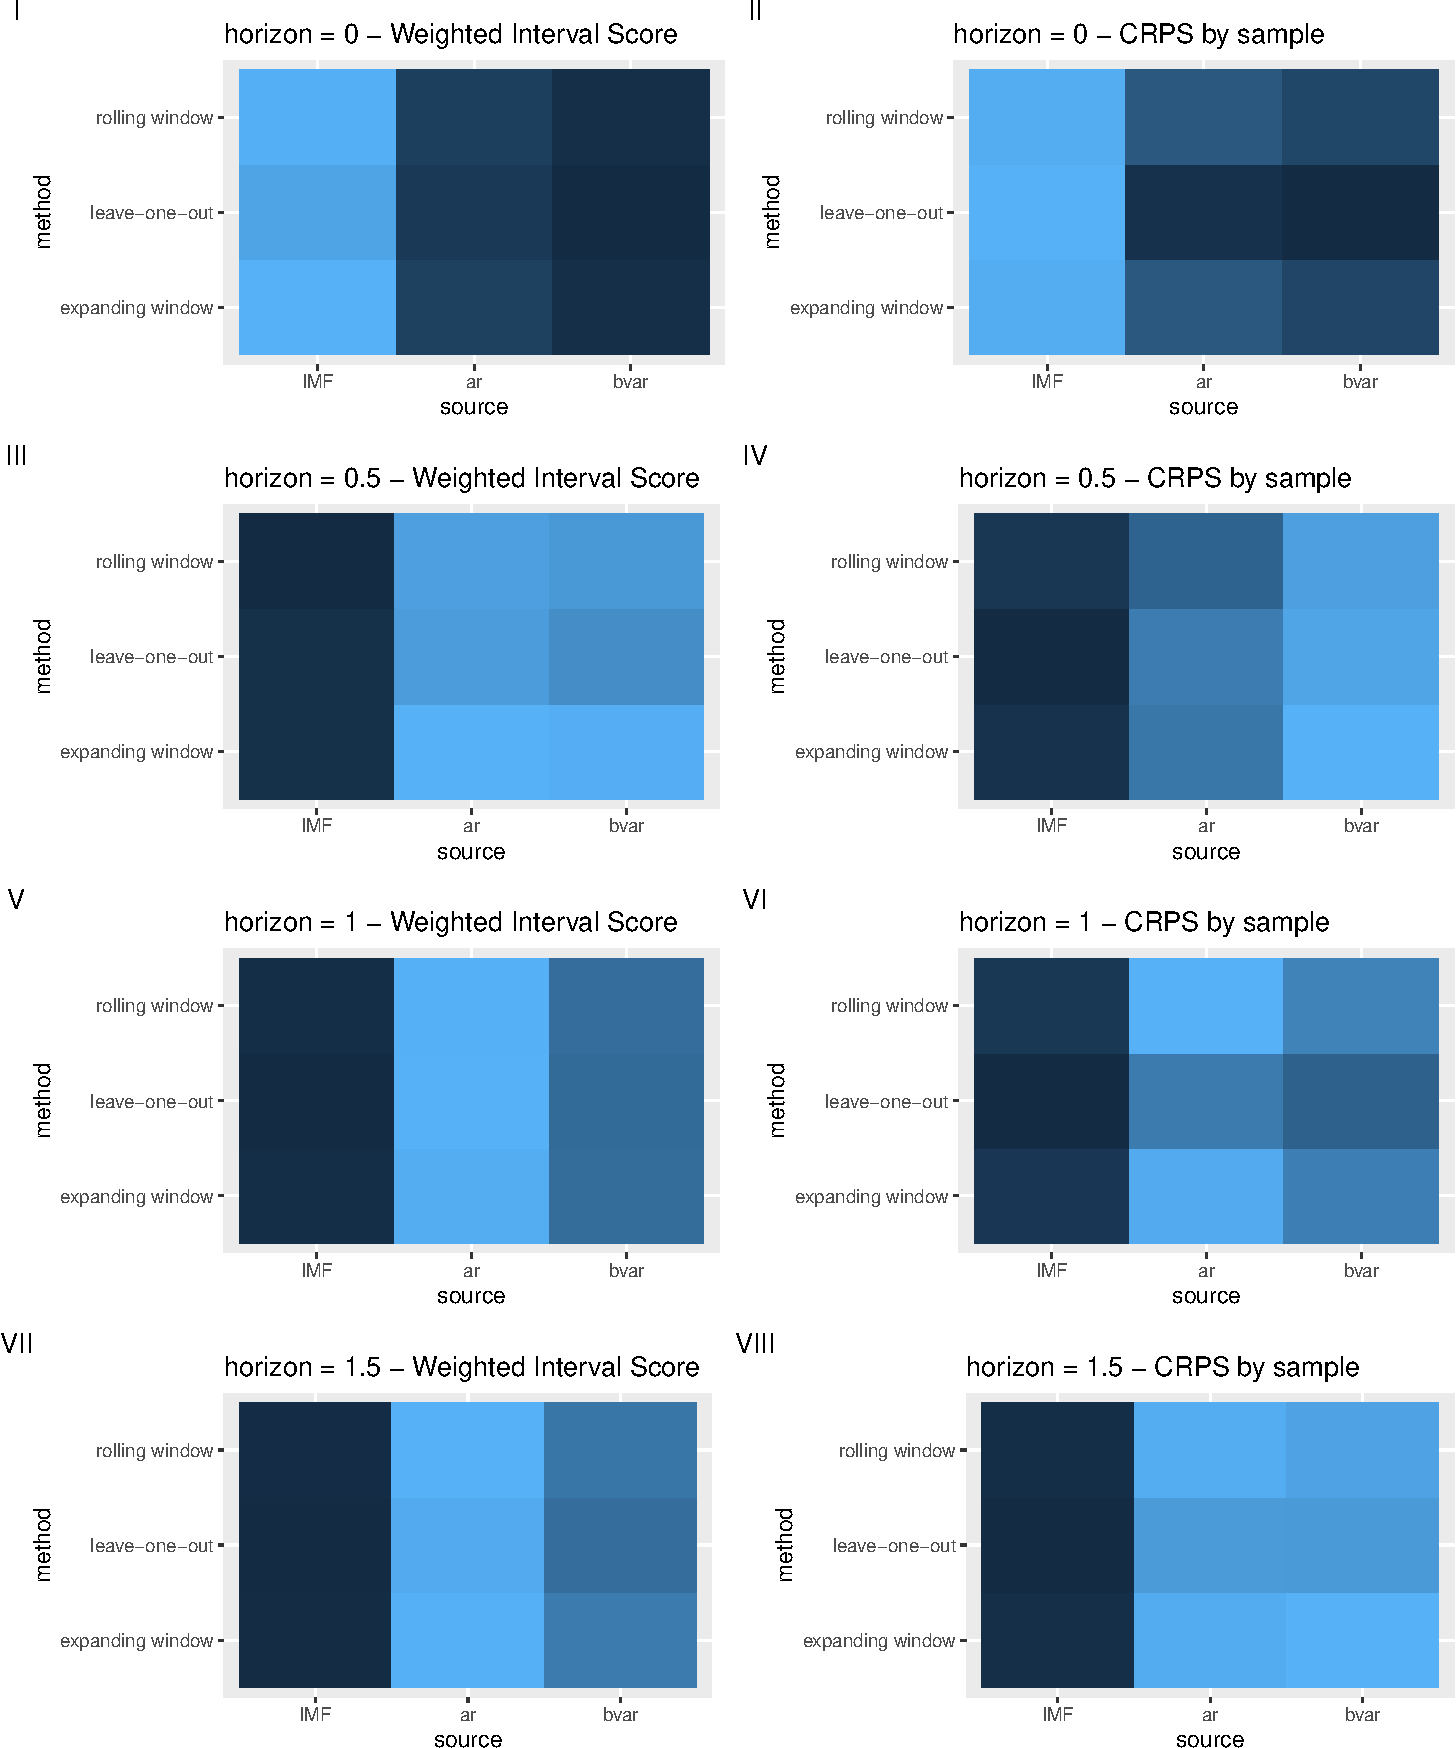
\includegraphics{manuscript_files/figure-latex/cpitileplot-1.pdf}

\hypertarget{gdp-2}{%
\subsection{GDP}\label{gdp-2}}

\begin{longtable}{l|rrr}
\toprule
\multicolumn{1}{l}{} & IMF & ar & bvar \\ 
\midrule\addlinespace[2.5pt]
\multicolumn{4}{l}{horizon = 0} \\ 
\midrule\addlinespace[2.5pt]
expanding window\_interval\_score & 0.241 & 0.301 & 0.298 \\ 
expanding window\_sample\_crps & 0.178 & 0.209 & 0.204 \\ 
leave-one-out\_interval\_score & 0.235 & 0.297 & 0.295 \\ 
leave-one-out\_sample\_crps & 0.183 & 0.219 & 0.214 \\ 
rolling window\_interval\_score & 0.240 & 0.302 & 0.297 \\ 
rolling window\_sample\_crps & 0.178 & 0.211 & 0.204 \\ 
\midrule\addlinespace[2.5pt]
\multicolumn{4}{l}{horizon = 0.5} \\ 
\midrule\addlinespace[2.5pt]
expanding window\_interval\_score & 0.416 & 0.540 & 0.493 \\ 
expanding window\_sample\_crps & 0.298 & 0.383 & 0.358 \\ 
leave-one-out\_interval\_score & 0.406 & 0.532 & 0.482 \\ 
leave-one-out\_sample\_crps & 0.310 & 0.408 & 0.377 \\ 
rolling window\_interval\_score & 0.416 & 0.554 & 0.504 \\ 
rolling window\_sample\_crps & 0.297 & 0.405 & 0.373 \\ 
\midrule\addlinespace[2.5pt]
\multicolumn{4}{l}{horizon = 1} \\ 
\midrule\addlinespace[2.5pt]
expanding window\_interval\_score & 0.846 & 1.094 & 0.947 \\ 
expanding window\_sample\_crps & 0.640 & 0.822 & 0.763 \\ 
leave-one-out\_interval\_score & 0.833 & 1.083 & 0.933 \\ 
leave-one-out\_sample\_crps & 0.634 & 0.759 & 0.709 \\ 
rolling window\_interval\_score & 0.858 & 1.121 & 0.973 \\ 
rolling window\_sample\_crps & 0.663 & 0.875 & 0.815 \\ 
\midrule\addlinespace[2.5pt]
\multicolumn{4}{l}{horizon = 1.5} \\ 
\midrule\addlinespace[2.5pt]
expanding window\_interval\_score & 1.063 & 1.297 & 1.113 \\ 
expanding window\_sample\_crps & 0.790 & 0.937 & 0.897 \\ 
leave-one-out\_interval\_score & 1.030 & 1.292 & 1.109 \\ 
leave-one-out\_sample\_crps & 0.765 & 0.882 & 0.849 \\ 
rolling window\_interval\_score & 1.075 & 1.313 & 1.150 \\ 
rolling window\_sample\_crps & 0.831 & 0.985 & 0.949 \\ 
\bottomrule
\end{longtable}

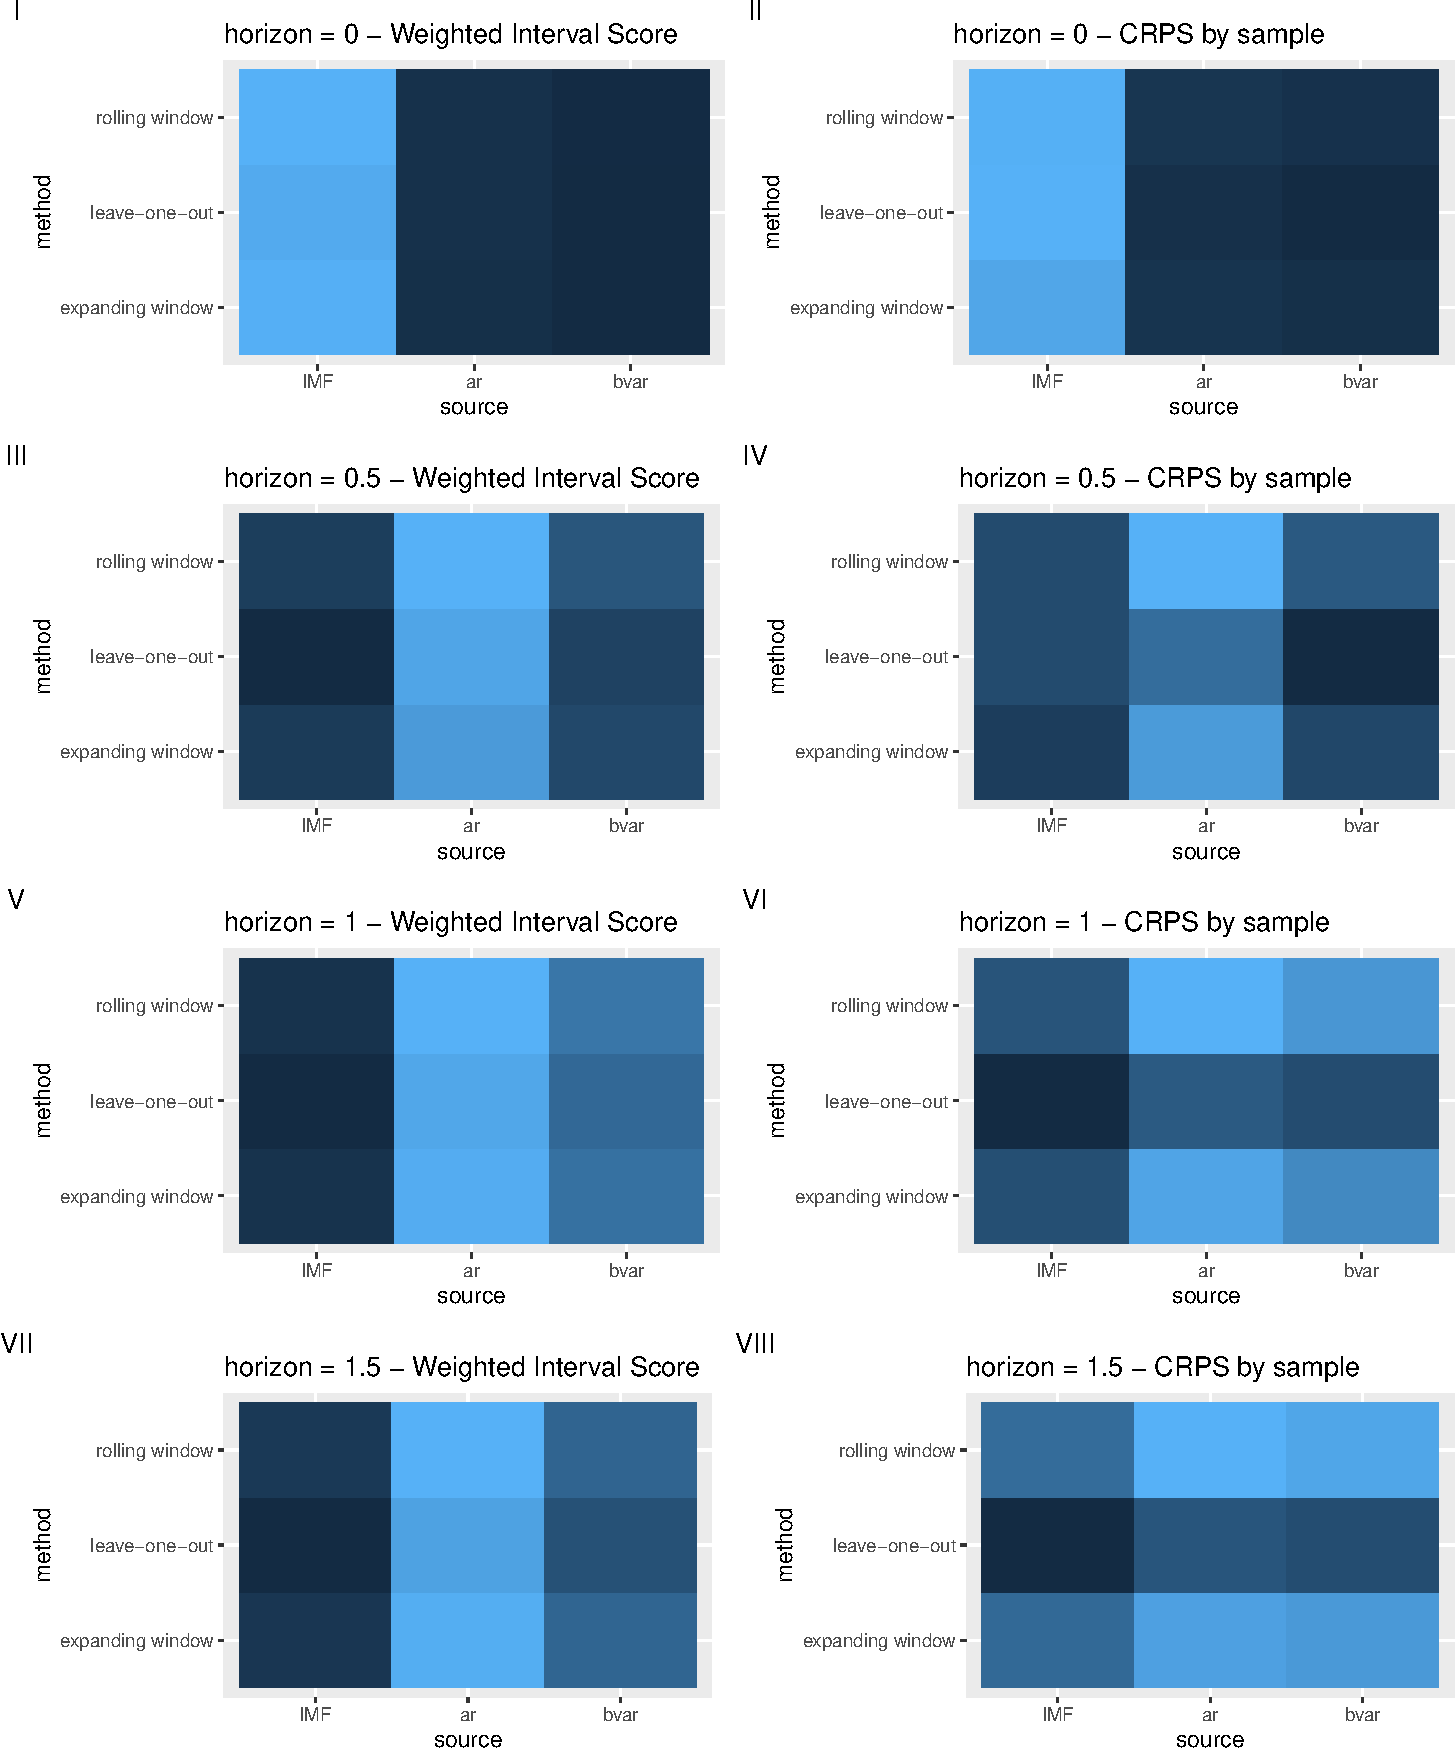
\includegraphics{manuscript_files/figure-latex/gdptileplot-1.pdf}

\end{document}
